At some MRPs and off-policy distributions, it may not be possible for regularization to ever do better than the error from learning that all states have zero value. We call these examples \emph{vacuous}.
%\begin{center}
%    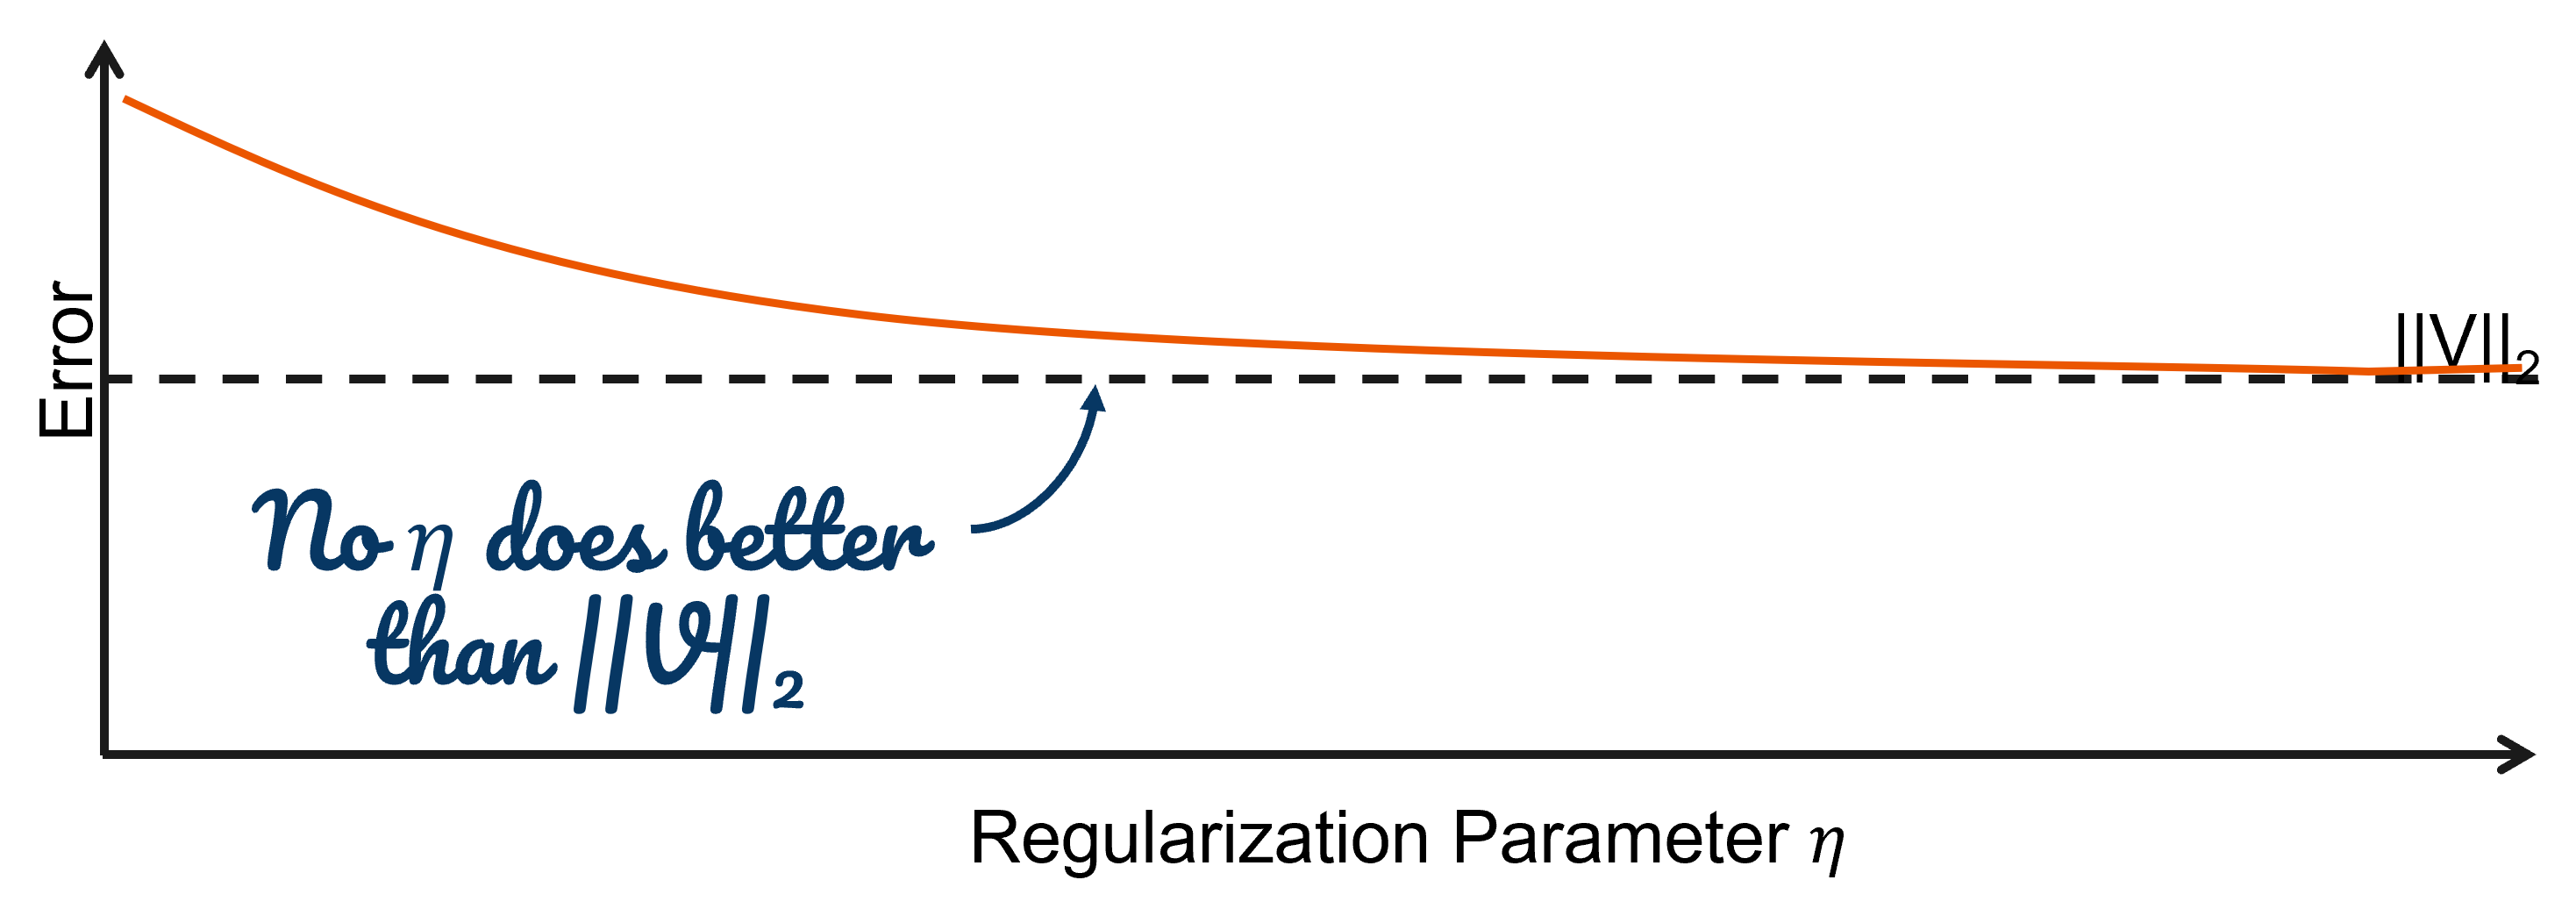
\includegraphics[scale=0.4]{parts/vacuous/vacuous.png}
%\end{center}
In our three-state example TD learns at vacuous value function at a specific off-policy distribution:
\begin{center}
    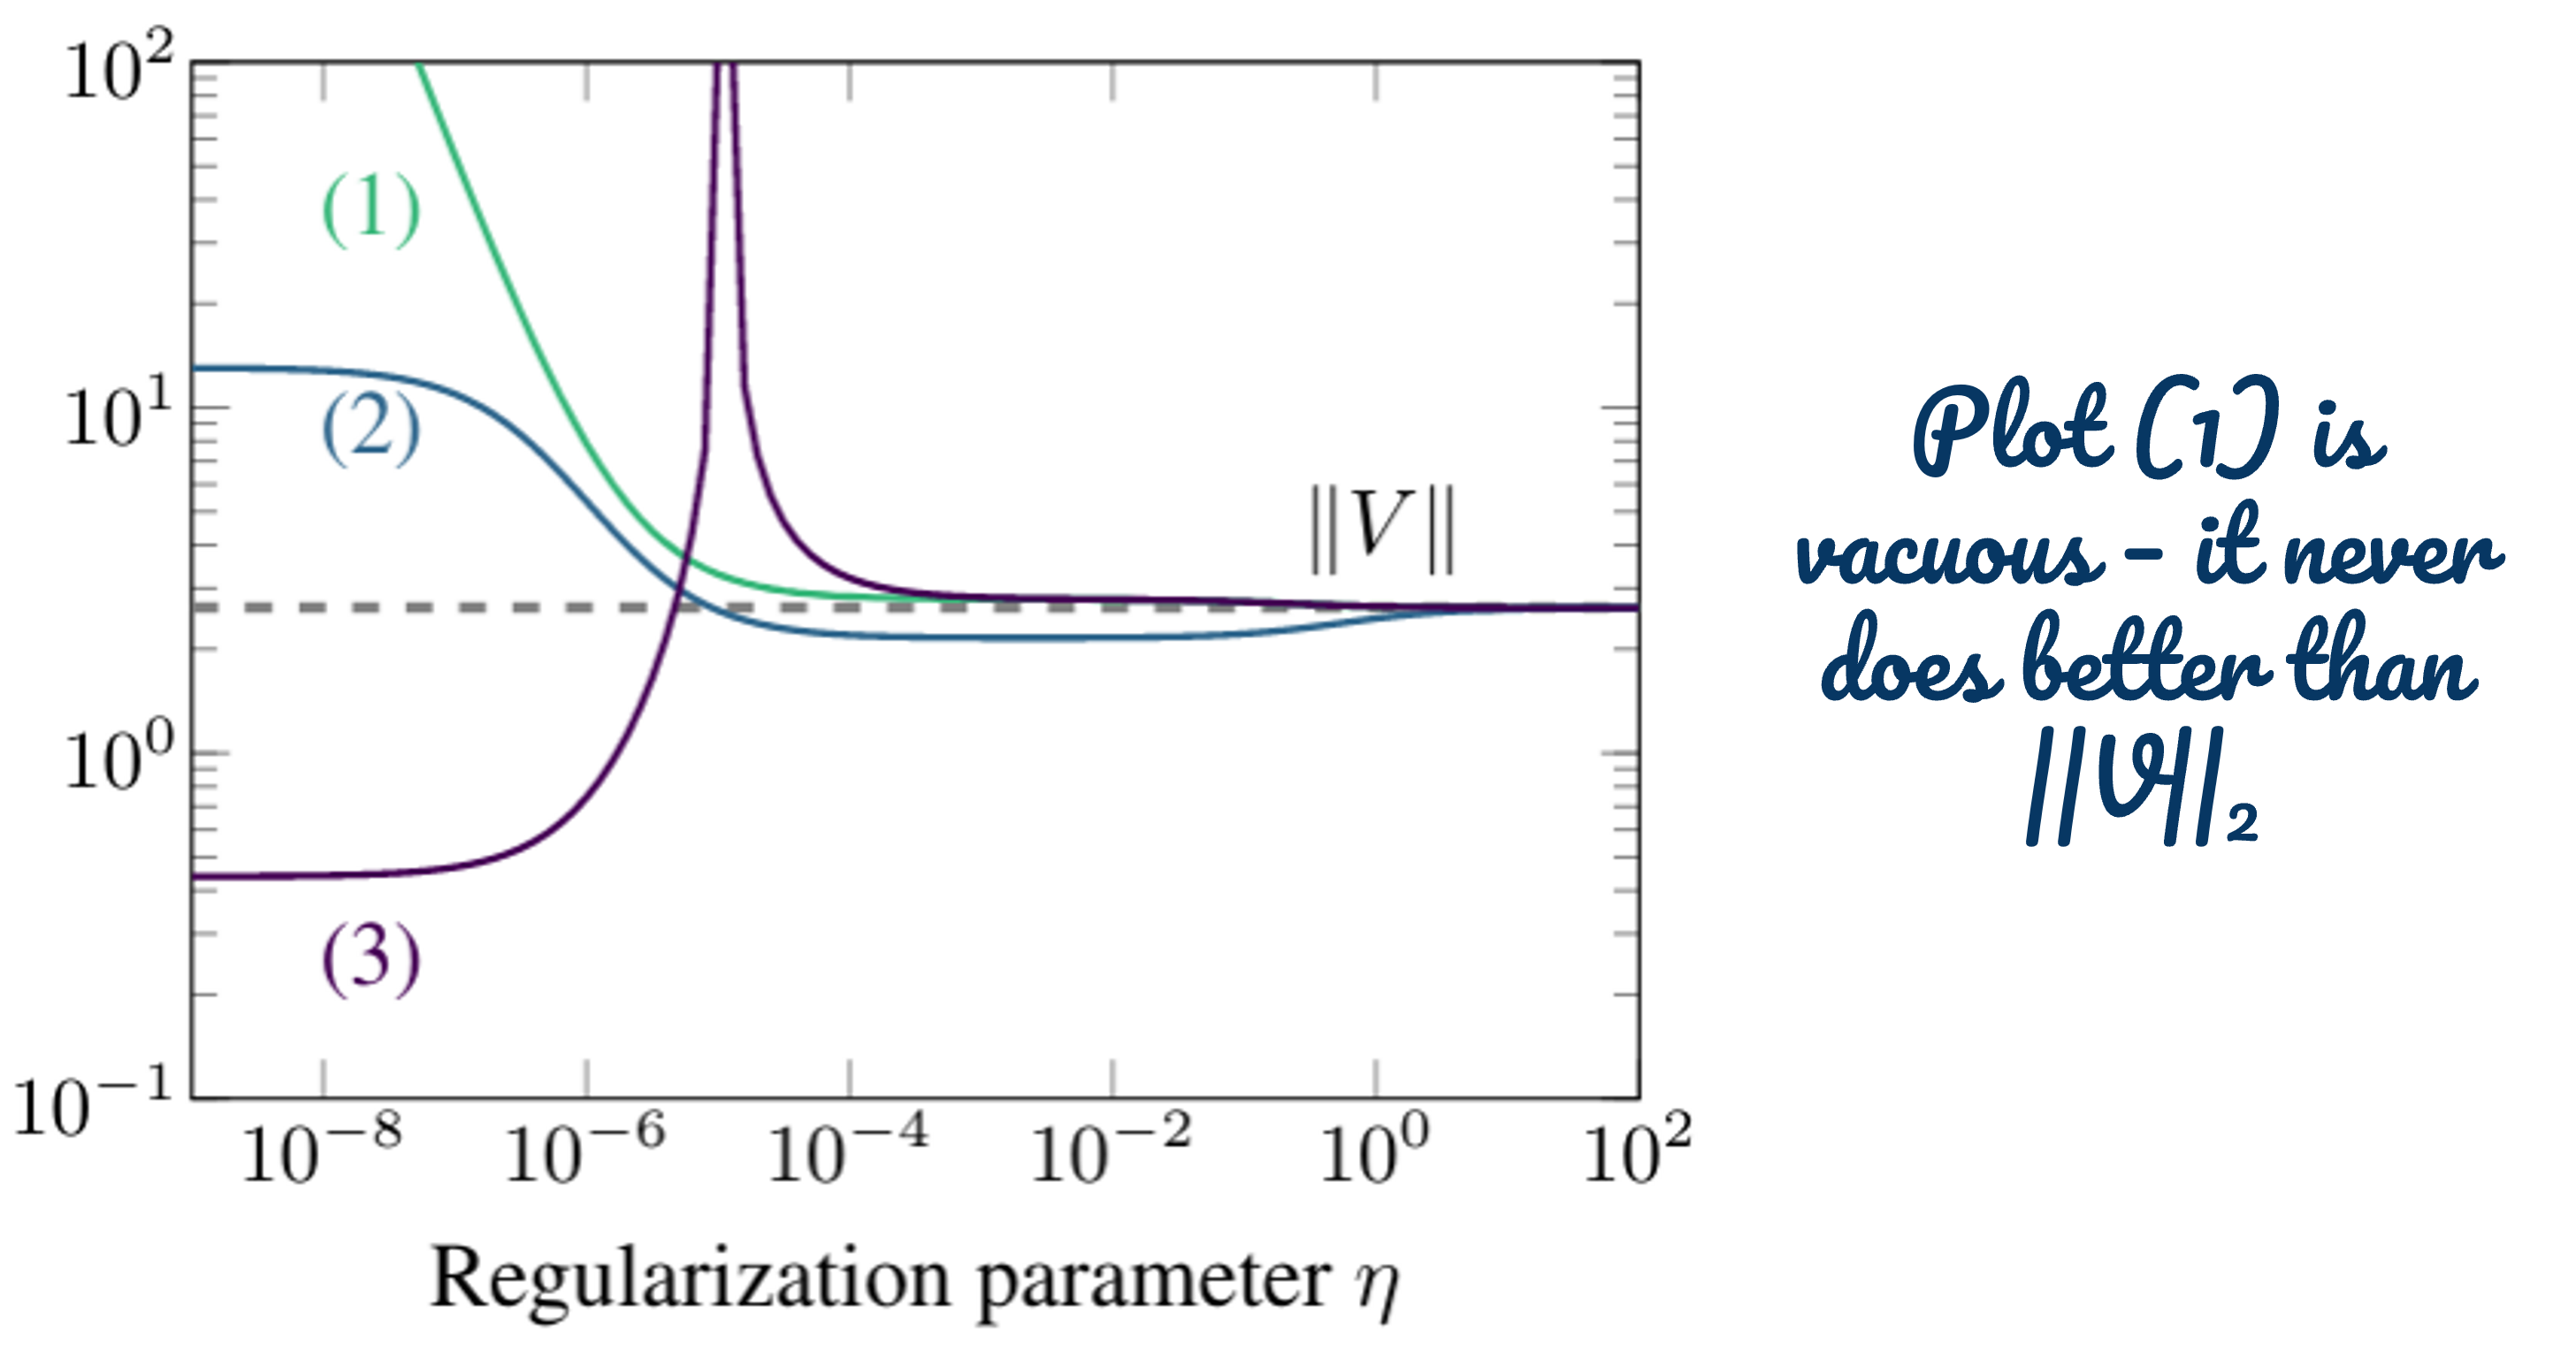
\includegraphics[scale=0.4]{parts/vacuous/vacuousactual.png}
\end{center}
\vspace{-.5in}
